\chapter{How I Turned \$50{,}000 Into \$20 Billion}

This lecture begins with an almost comic compression. We are told that we are meeting one of the richest men in the world, and then the answer comes back in plain language: he sells chicken fingers. The chapter that follows keeps that rhythm. We begin with the paradox of enormous scale built on a narrow product, move backward to rejection and first funding, then forward through leverage, focus, ownership, and thin-margin unit economics. No validated screenshots survived for this lecture, so every diagram here is a transcript-derived reconstruction rather than a transcription of visible board work.

\section{The Billionaire Chicken-Finger Paradox}

The opening is not merely promotional framing. It identifies the central puzzle of the lecture: how can a business that sounds so narrow carry such large scale? The host places us at the original Raising Cane's location in Baton Rouge, and that move matters. The first store is not background scenery; it is the initial condition from which the entire later expansion must be understood.

The lecture then places three numerical markers on the table. They do not explain the machine by themselves, but they tell us the size of the machine we are trying to understand:
\begin{equation}
W > \$20\times 10^{9},\qquad N>900,\qquad Y_{\max}\approx \$4\times 10^{8}.
\end{equation}
Here \(W\) denotes reported net worth, \(N\) the number of locations, and \(Y_{\max}\) the reported best single-year earnings figure cited in the interview.

The important structural point is that the lecture does not begin with abstract theory. It begins with a mismatch between appearance and scale. Only after that mismatch is clear do we return to the origin story.

\section{Rejection Before Proof}

\paragraph{Anecdote.}
Todd Graves describes a childhood already oriented toward small enterprise: lemonade stands, cutting grass, and then restaurant work in high school and college. In college he presented a business plan centered on chicken fingers and received the lowest grade in the class. The plan itself, as he tells it, was not the problem; the professor rejected the concept. A restaurant built around a single narrow item was judged implausible precisely when other chains were broadening menus.

\paragraph{Claim.}
The lecture's first serious claim is that rejection does not settle the matter. In the spoken rhythm of the interview, rejection is not interpreted as information from the market; it is treated as an external judgment delivered \emph{before} the market has spoken.

\subsection{Question \& Answer}

\paragraph{Question.}
What are we supposed to do with rejection before we have any credibility at all?

\paragraph{Answer.}
Graves's answer is not subtle: use it as fuel. That answer can sound merely motivational unless we keep the context. He is speaking specifically about the interval before proof, when the entrepreneur has neither numbers from a running business nor reputation from prior wins. In that interval, the only available capital may be conviction joined to work.

The lecture's logic can be written in deliberately minimal form:
\begin{equation}
\text{early rejection} \not\Rightarrow \text{false model}.
\end{equation}
This is not a theorem of business, and the lecture does not pretend that every dismissed idea will succeed. The narrower point is different: classroom disbelief and social refusal are not yet the same thing as operational disproof.

\paragraph{Mechanism.}
The mechanism here is psychological but not vague. A person either lets refusal collapse effort, or he converts refusal into additional persistence. The interview keeps that tension alive because the next obstacle is harder. It is one thing to survive mockery; it is another to finance a capital-intensive first store.

\section{Financing the First Store}

\paragraph{Anecdote.}
The host asks the right next question. Restaurant businesses are capital-intensive, and the banks were not lending to him. Graves's answer is brutally concrete: if the bank will not finance the experiment, then the founder must first make himself financeable. In his case that meant physically difficult work, including commercial fishing in Alaska, followed by the use of government-backed entrepreneurial programs once enough personal equity had been raised.

\paragraph{Claim.}
The lecture's claim is that a first capital stack need not arrive all at once from a single lender. It can be assembled in stages:
\begin{align}
K_0 &= E_0 + L_0,\\
E_0 &\approx \$50{,}000,\qquad L_0 \approx \$50{,}000,\\
K_0 &\approx \$100{,}000.
\end{align}
Here \(K_0\) is the capital available to open the first store, \(E_0\) is founder equity raised through labor and saving, and \(L_0\) is the later SBA-backed loan.

\begin{figure}[h]
\centering
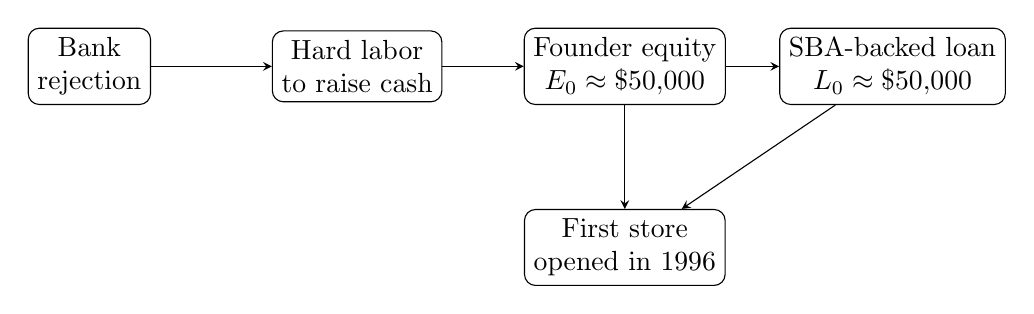
\begin{tikzpicture}[>=stealth, node distance=1.9cm]
\node[draw, rounded corners, align=center] (a) {Bank\\rejection};
\node[draw, rounded corners, align=center, right of=a, xshift=1.5cm] (b) {Hard labor\\to raise cash};
\node[draw, rounded corners, align=center, right of=b, xshift=1.5cm] (c) {Founder equity\\\(E_0\approx \$50{,}000\)};
\node[draw, rounded corners, align=center, right of=c, xshift=1.5cm] (d) {SBA-backed loan\\\(L_0\approx \$50{,}000\)};
\node[draw, rounded corners, align=center, below of=c, yshift=-0.4cm] (e) {First store\\opened in 1996};

\draw[->] (a) -- (b);
\draw[->] (b) -- (c);
\draw[->] (c) -- (d);
\draw[->] (c) -- (e);
\draw[->] (d) -- (e);
\end{tikzpicture}
\end{figure}

\paragraph{Mechanism.}
The mechanism is cumulative. First one earns money directly. Then one uses that equity to make the business legible to a lender. Then one supplements equity with debt. The lecture also mentions public small-business support structures. Because the transcript is slightly noisy on exact institutional names, it is best to record the point cautiously: Graves used government-backed lending and small-business advisory resources as part of the path from idea to opening day.

\subsection{Question \& Answer}

\paragraph{Question.}
How does one start a capital-intensive business when ordinary banks say no?

\paragraph{Answer.}
The answer given here is not to wait for universal approval. It is to reduce the distance between idea and fundability. One raises some money personally, one learns the business closely, one uses public entrepreneurial infrastructure where available, and only then asks the bank to finance a smaller and more defensible gap.

\section{Know the Numbers, Then Negotiate}

Once the first capital stack is in place, the lecture turns from money to argument. The host asks what Graves learned about negotiating with banks, and the answer is numerical rather than theatrical. One must know the numbers well enough to defend the low, medium, and high cases.

The lecture's forecast structure may be written as
\begin{align}
\Pi_{\mathrm{low}} &\approx 0,\\
\Pi_{\mathrm{med}} &> 0,\\
\Pi_{\mathrm{high}} &> \Pi_{\mathrm{med}}.
\end{align}
The language is informal, but the structure is clear. The low case is the break-even or survival case. The medium case is the ordinary profitable case. The high case is the stronger case in which the loan may be repaid more quickly.

\paragraph{Worked forecast logic.}
\begin{enumerate}
\item The downside case must not be fantasy. It must show that the business can survive even when things are merely adequate.
\item The middle case must show that the business is economically worth doing, not simply capable of avoiding collapse.
\item The high case is not there to impress; it is there to demonstrate the lender's upside through faster repayment.
\item If one lender rejects a set of numbers that the founder genuinely understands and believes, Graves's advice is not to falsify the numbers but to take them elsewhere.
\end{enumerate}

The lecture's negotiation principle can be summarized as
\begin{equation}
\Pi_{\mathrm{low}} \ge 0
\quad\Longrightarrow\quad
\text{the business survives the downside state.}
\end{equation}
That is the core underwriting intuition in the interview. The high case is attractive, but the low case must still make operational sense.

\paragraph{Interruption.}
At this point the original video is interrupted by a long host-side promotional segment about his own network and paid community. For our purposes that interruption should be bracketed. It belongs to the video's monetization rhythm, not to Graves's line of financial reasoning. When the interview resumes, the tone becomes harsher: the next lesson is not about getting the first loan, but about nearly breaking the business with too much debt.

\section{Leverage, Shock, and Scale by Focus}

\paragraph{Anecdote.}
Graves says plainly that he almost broke the business by overleveraging it while growing. Then Hurricane Katrina hit, and between \(21\) and \(28\) restaurants went down. The crucial point is that the debt did not go down merely because revenue capacity did.

\paragraph{Claim.}
The lecture's anti-fragility lesson is simple. If a shock removes operating capacity while fixed financial obligations remain, leverage becomes dangerous. In minimal notation we may write
\begin{align}
N_{\mathrm{eff}} &= N - N_{\mathrm{down}},\\
N_{\mathrm{down}} &\in [21,28].
\end{align}
If effective operating scale falls but bank obligations remain fixed, the business is squeezed from both sides.

This is not a full balance-sheet model, because the lecture does not give one. But the direction is clear enough:
\begin{equation}
R_{\mathrm{eff}}\downarrow \qquad \text{while} \qquad DS \ \text{does not automatically fall.}
\end{equation}
Here \(R_{\mathrm{eff}}\) is effective revenue after disruption and \(DS\) is debt service.

\paragraph{Mechanism.}
The mechanism of the lesson is retrospective. Debt accelerates normal growth, but it also narrows the margin of survival under external shock. Hence the later rule: do not overleverage; grow with more equity.

The interview then pivots directly from fragility to scaling. That transition matters. Graves does not say, ``therefore avoid growth.'' He says, in effect, ``grow, but grow correctly.'' The operating secret is not diversification first. It is focus first.

The lecture condenses that operating doctrine into a single sequence:
\begin{equation}
1 \longrightarrow 10 \longrightarrow 100 \longrightarrow 900+.
\end{equation}
The arrow here does not mean expansion by menu breadth. It means replication of a narrow, strong operating unit.

\begin{figure}[h]
\centering
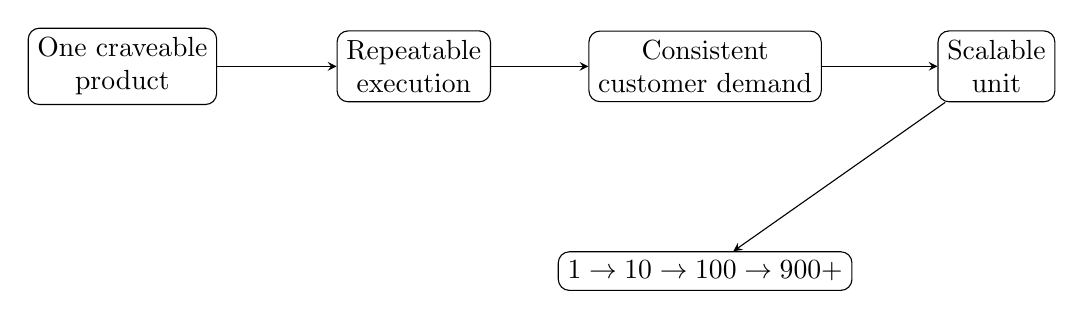
\begin{tikzpicture}[>=stealth, node distance=2.2cm]
\node[draw, rounded corners, align=center] (a) {One craveable\\product};
\node[draw, rounded corners, align=center, right of=a, xshift=1.5cm] (b) {Repeatable\\execution};
\node[draw, rounded corners, align=center, right of=b, xshift=1.5cm] (c) {Consistent\\customer demand};
\node[draw, rounded corners, align=center, right of=c, xshift=1.5cm] (d) {Scalable\\unit};
\node[draw, rounded corners, align=center, below of=c, yshift=-0.4cm] (e) {\(1\to 10\to 100\to 900+\)};

\draw[->] (a) -- (b);
\draw[->] (b) -- (c);
\draw[->] (c) -- (d);
\draw[->] (d) -- (e);
\end{tikzpicture}
\end{figure}

\subsection{Question \& Answer}

\paragraph{Question.}
Why not diversify, especially when outsiders keep saying that broader menus and more variety are safer?

\paragraph{Answer.}
Because, as Graves puts it, trying to be all things to all people satisfies nobody. The lecture's scaling logic is that a narrow product can become large if it is sufficiently craveable and executed exceptionally well. Variety may increase the menu, but it may also dilute the operating identity that made the first unit powerful enough to repeat.

\section{Ownership, Competition, and the Long Run}

The next movement of the lecture asks who gets to make decisions once the business is large. Graves says he owns roughly \(91\%\) to \(92\%\) of the company:
\begin{equation}
s_{\mathrm{Todd}} \approx 0.91\text{--}0.92.
\end{equation}
That number is not presented as vanity. It is presented as a control variable.

In the transcript, the practical meaning of control is immediate. If outside owners have different intentions, they may force short-term decisions that improve a quarter and weaken the enterprise. Because Graves holds control, he says he can avoid certain reactions in bad years: he need not cut wages merely to defend the near-term statement, and he need not raise prices reflexively.

A cautious editorial way to formalize his point is
\begin{equation}
\max \sum_{t\ge 0}\delta^t \Pi_t
\qquad \text{rather than} \qquad
\max \Pi_0.
\end{equation}
This is our notation, not his. But it captures the logic of the interview: ownership concentration can permit a longer decision horizon.

The lecture then adds a second ingredient: competition. Graves says he likes competition because it sharpens execution. This is consistent with the rest of the chapter. A founder who believes the unit is strong does not necessarily interpret competition as disproval. He may interpret it as an invitation to work harder.

Finally, the host asks the obvious question: why continue after very large wealth has already been achieved? The answer is purpose. In the interview, wealth does not end the game; it changes the scale on which service and impact can be imagined. The internal chronology is important. First comes product, then scale, then ownership, then long-horizon purpose. The lecture does not begin with moral language; it arrives there after the machine has already been built.

\section{Purpose, Progress, and the Arithmetic of Thin Margins}

This last large section braids together three themes that the lecture treats as connected: service, iteration, and unit economics.

\paragraph{Anecdote.}
The purpose language in the lecture is explicit. The business is said to exist not simply to enrich its owner but to provide jobs, build a place people want to work, and create resources that can flow back into communities. The leadership rule that follows is therefore unsurprising: lead by example, believe in people, take care of people, and understand that to lead is to serve.

The next beat deepens the operating side. Graves says he learned from a mentor to prefer progress over perfection. His example is concrete. A training manual delayed until perfect becomes a brake on the business.

\subsection{Question \& Answer}

\paragraph{Question.}
What matters more in a growing business: perfection or progress?

\paragraph{Answer.}
The lecture answers by way of iteration. Release the first workable version, then improve it. In our notation,
\begin{equation}
v_1 \longrightarrow v_2 \longrightarrow \cdots \longrightarrow v_{100}.
\end{equation}
The point is not that early versions are good enough in every absolute sense. The point is that an operating business learns through revision. Perfectionism can halt the flow of learning by refusing to publish version \(1\).

\paragraph{Mechanism.}
The mechanism is cumulative improvement. One ships a training program, gathers experience, revises it, and repeats. This is not far from the earlier logic of the restaurant itself. One strong unit is refined and replicated. The lecture's repeated insistence on fanatic commitment and high risk tolerance belongs here as well. Iteration is not gentle. It is sustained effort under pressure.

The coda of the lecture returns us to the table and therefore to the business's most material fact: margins are thin. The menu has remained stable for decades, the sauce remains operationally controlled, and the arithmetic is tight:
\begin{align}
\Pi &= \mu R,\\
\mu &\in [0.05,0.10].
\end{align}
Here \(\mu\) is the profit margin per dollar of revenue, interpreted from the statement that margins are roughly five to ten cents on the dollar when things are going very well.

This gives the lecture's final operational lesson. If margin is small, then serious profit requires very large revenue:
\begin{equation}
R^* = \frac{\Pi^*}{\mu}.
\end{equation}

\paragraph{Worked example.}
Suppose a store or group of stores targets
\[
\Pi^* = \$1{,}000{,}000.
\]
Then:
\begin{align}
R^*(\mu=0.05) &= \frac{\$1{,}000{,}000}{0.05} = \$20{,}000{,}000,\\
R^*(\mu=0.10) &= \frac{\$1{,}000{,}000}{0.10} = \$10{,}000{,}000.
\end{align}
So the lecture's closing slogan, ``push the top line and be smart with the bottom line,'' is not just rhetoric. It is the arithmetic of a thin-margin business. Quality and service may cost money, but if they materially increase repeat demand, they can enlarge \(R\) enough to justify the discipline.

\paragraph{A final business reconstruction.}
At the end of the lecture, if we compress the machine into one line, it looks like this:
\begin{equation}
\text{focus} + \text{execution} + \text{volume} + \text{time} \longrightarrow \text{scale}.
\end{equation}
That line is schematic, but it is faithful to the chapter's progression. We have moved from one store, to a repeated unit, to a controlled operating system, to a business where the economics live in volume because the margin on each dollar is narrow.

\section{Summary}

The lecture never presents a single grand formula for becoming wealthy, and it would be a mistake to force one onto it. What it does present is a coherent sequence.

First, a narrow product can scale if it is strong enough to repeat. Second, early rejection is not yet market disproof. Third, first capital may have to be assembled in stages, with labor creating equity and equity creating fundability. Fourth, numerical discipline matters because lenders care about downside survival, not just upside enthusiasm. Fifth, overleverage turns growth fragile under shock. Sixth, concentrated ownership can protect long-horizon decisions. Finally, thin margins mean that quality, service, and volume are not separate topics; they are part of one operating equation.

That is why the lecture ends at the table rather than in abstraction. The billionaire story returns to the box combo, the unchanged menu, and the stubborn arithmetic of a business that makes only a few cents on the dollar and therefore must be both excellent and enormous.